\documentclass[a4paper,11pt]{article}
\usepackage[a4paper,total={18cm, 24cm}]{geometry}
\usepackage[parfill]{parskip}
\usepackage[utf8]{inputenc}
\usepackage[T1]{fontenc}
\usepackage{fancyhdr}
\usepackage[ddmmyyyy]{datetime}
\usepackage{graphicx}
\usepackage{subcaption}
\usepackage{multirow}
\usepackage{hyperref}

\pagestyle{fancy}
\fancyhf{}
\lhead{\today}
\chead{Deep Learning - Transfer Learning and Fine Tuning}
\rhead{Jakub Rada}

\begin{document}
In this assignment we explored convolutional neural networks and especially fine tuning and transefer learning.
We use two \textit{State of the Art} pretrained models, \textbf{SqueezeNet} and \textbf{ResNet-18}.
On the former we visualize convolutional neural networks to see how they work and on the latter we compare training from scratch, transfer learning and full fine tuning on a PAC cartoon dataset.

\section{SqueezeNet visualization}
As mentioned above, the first part of the assignment focuses on visualization of convolutional neural network to get an idea how they work on images.
To do this we used a pretrained \textbf{SqueezeNet} model and an image of a dog which can be seen in a figure \ref{fig:dog}.
Moreover, we have a list of names of classes which can be the output of the network.
Note that this part is implemented in a Python file \textit{01\_squeezenet.py}.

\begin{figure}[ht]
    \centering
    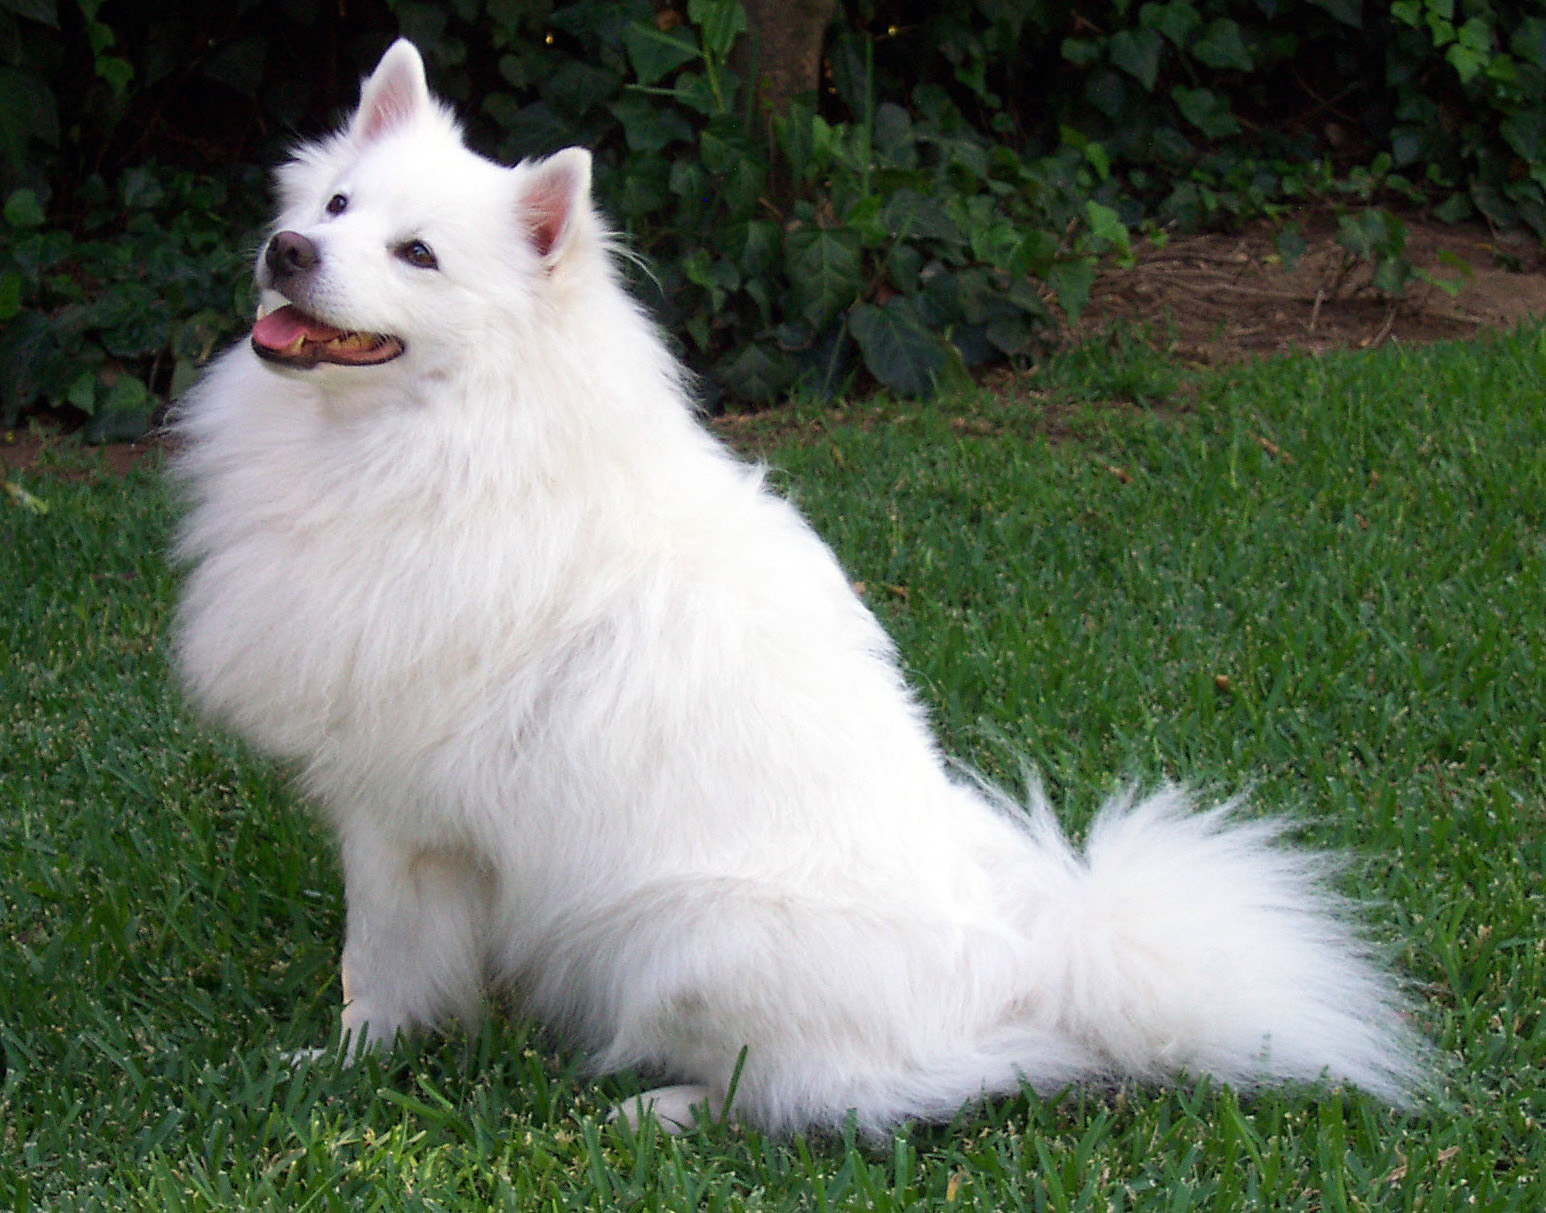
\includegraphics[width=0.4\textwidth]{../data/dog.jpg}
    \caption{A dog used for the first part}
    \label{fig:dog}
\end{figure}

In order for the network to classify it correctly, we must ensure correct format of the image, which is shape (channels, height, width).
Also, we need to provide the RGB values (3 channels) either in float range $[0, 1]$ or integer range $[0, 255]$.

\paragraph*{Prediction} First, we fed this image to the neural network and try to classify it.
We list the top classes with prediction probabilities in the following table \ref{table:dog}.

\begin{table}[ht]
    \centering
    \begin{tabular}{|c|c|}
        \hline
        \textbf{Class}              & \textbf{Probability / Confidence} \\
        \hline
        \hline
        Samoyed                     & 95.04\%                           \\
        malamute                    & 0.84\%                            \\
        Pomeranian                  & 0.74\%                            \\
        collie                      & 0.56\%                            \\
        West Highland white terrier & 0.46\%                            \\
        \hline
    \end{tabular}
    \caption{Top-5 predicted classes for the dog image}
    \label{table:dog}
\end{table}

We can see that the network predicted the correct (in my opinion, according to images of Samoyeds) class with a very high confidence.
The other 4 classes from top-5 have tiny probabilities.

\paragraph*{Weights of convolutional layer} Next, we want to visualize the weights of the first convolutional layer of the network to perhaps see some detected patterns.
The first convolutional layer has 96 channels of size $3 \times 7 \times 7$, where 3 is the number of colors and 7's are the spatial dimensions of the individual filters.
The channels are visualized in the figure \ref{fig:cnn-weights} organized into a $8 \times 12$ grid.

\begin{figure}[ht]
    \centering
    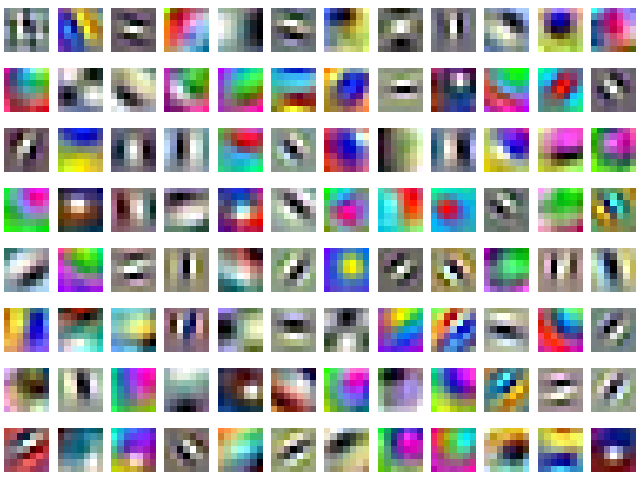
\includegraphics[width=0.75\textwidth]{../out/01_first_layer_weights.png}
    \caption{Weights of the first convolutional layer}
    \label{fig:cnn-weights}
\end{figure}

In the filters we can identify some edge detectors and simple color and small shape detectors.
We can confirm this in the last task of this part.

\paragraph*{Activation maps of the image} Last in this part, we visualize the activation maps of the dog image (\ref{fig:dog}) as it passes through the first convolutional layer.
We show only the first 16 channels ($4 \times 4$ grid) before and after \textit{ReLU} non-linearity in \ref{fig:activation-maps}.

\begin{figure}[ht]
    \centering
    \hfill
    \begin{subfigure}[b]{0.4\textwidth}
        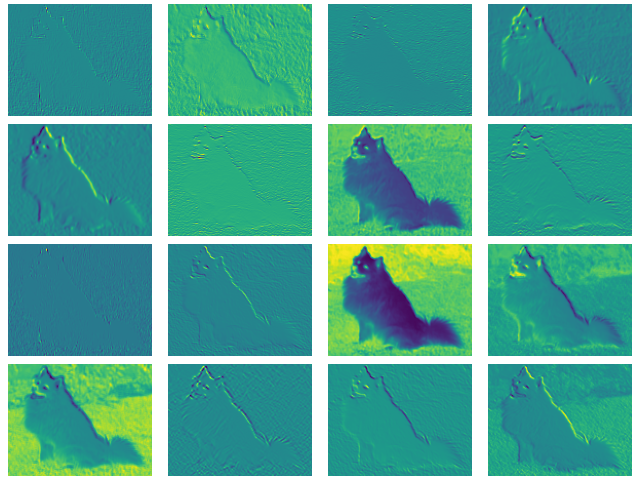
\includegraphics[width=\textwidth]{../out/01_pass_first_layer.png}
        \caption{Activation maps before \textit{ReLU}}
    \end{subfigure}
    \hfill
    \begin{subfigure}[b]{0.4\textwidth}
        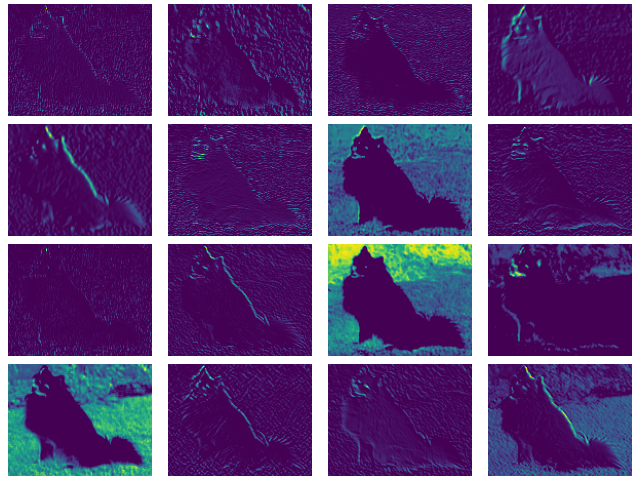
\includegraphics[width=\textwidth]{../out/01_pass_first_layer_activated.png}
        \caption{Activation maps after \textit{ReLU}}
    \end{subfigure}
    \hfill
    \caption{Activation maps of the dog image after first convolutional layer}
    \label{fig:activation-maps}
\end{figure}

From these images we can see that indeed, some filters detect edges in the image, some of them detect the background behind the dog and similar things.
Some of them slightly blur the dog, while other preserve sharpness, some of them preserve the texture more than others.
It corresponds to the notion, that the first layers detect simple, atomic patterns and then they are combined into more high-level features in deeper layers.

\section{Transfer learning and fine tuning}
In the previous section, we visualized the first layer of a simple convolutional model \textbf{SqueezeNet} and how it extracts features from an image.
In this sectin, we will take a more complex model and compare three learning approaches on a cartoon dataset.
Later, we will compare these methods also on a smaller dataset with fewer training data to see how well they perform when we have only limited data.

This part is implemented in a Python file \textit{02\_resnet.py} and consists of slightly general functions which enabled me to conduct experiments in an easy way.
Most importantly, I have a function \textit{cross\_validate} which takes a model building method as one of the parameters and, of course, learning parameters and executes the standard learning loop.
The building functions correspond to the three learning approaches we want to compare.
Also, I tried to maximize similarity between the experiments, so I initialized the loaders with the same seed before every experiment.
This ensures (not only) that the split into \textit{training} and \textit{validation} sets is the same.

\subsection{Full PACS cartoon dataset}

\subsubsection{Preprocessing}
To improve learning during training, it is a good idea to normalize the data so that they have $0$ mean and $1$ variance.
We accomplish this by computing the statistics of the training set and then using PyTorch \textit{transforms} to normalize the datasets.
The statistics should be computed efficiently in batches, which I tried to do in the code.
The values I got for the \textit{PACS\_cartoon} training set is shown in the table \ref{table:stats}.

\begin{table}[ht]
    \centering
    \begin{tabular}{| r | c | c |}
        \hline
        Dataset                & Mean                       & Standard Deviation         \\
        \hline
        \hline
        \textbf{PACS\_cartoon} & $[0.8116, 0.7858, 0.7380]$ & $[0.2730, 0.2863, 0.3374]$ \\
        \hline
        \textbf{ImageNet}      & $[0.485, 0.456, 0.406]$    & $[0.229, 0.224, 0.225]$    \\
        \hline
    \end{tabular}
    \caption{Statistics of the training set comapred to \textbf{ImageNet}}
    \label{table:stats}
\end{table}

We see that the statistcs are not the same as in the \textit{ImageNet} dataset.

As mentioned above, the training set is partitioned into \textit{training} and \textit{validation} sets, where the \textit{validation} set is used to assess the quality of the model during training and is not used to compute gradients.
I chose the split ratio to be $0.8$ for the \textit{training} set and $0.2$ for the \textit{validation} for all of my experiments and the split was fixed by a seed value $42$.

\subsubsection{Training from scratch}
First, we train the model from scratch using only our own dataset.
We do it by using the \textbf{ResNet} model without downloading the weights.
We replace the classification layer of the original model with a new linear layer, which has $7$ output neurons and which is the number of classes we want to classify.
I initialized this new linear layer with \textit{xavier normal} random initialization provided by PyTorch.

Then, we train the network using cross-validation to find the best combination of learning rate\newline $\lambda \in \{0.01, 0.03, 0.001, 0.003, 0.0001\}$ and stopping epoch $e \in \{1, \dots, 50\}$.
As suggested in the template I used the \textit{SGD} optimizer, which has fixed learning rate during the whole optimization.
The table \ref{table:hyperparams} shows the summary of parameters used for training.

\begin{table}[ht]
    \centering
    \begin{tabular}{ | r | l | }
        \hline
        Learning rate $\lambda$                          & $\lambda \in \{0.01, 0.03, 0.001, 0.003, 0.0001\}$ \\
        \hline
        Stopping epochs $e$                              & $e \in \{1, ..., 50\}$                             \\
        \hline
        Optimizer                                        & SGD                                                \\
        \hline
        Validation set size (proportion of training set) & $0.2$                                              \\
        \hline
        Batch size                                       & 8                                                  \\
        \hline
        Seed (set before splitting the dataset)          & 42                                                 \\
        \hline
    \end{tabular}
    \caption{Training (hyper)-parameters}
    \label{table:hyperparams}
\end{table}

In each epoch, we go over the training dataset once and update weights by backpropagation.
After each epoch ends, we evaluate the network on the validation set and store the loss and accuracy.
We save the model with the best validation accuracy and remember the learning rate and epoch.
Later, we will use this best model to evaluate it on the test set, which is completely separate from the two other sets and is left untouched by training.

In the graph \ref{fig:full_scratch}, I show the training and validation loss and accuracy for all the learning rates depending on the epoch.

\begin{figure}[ht]
    \centering
    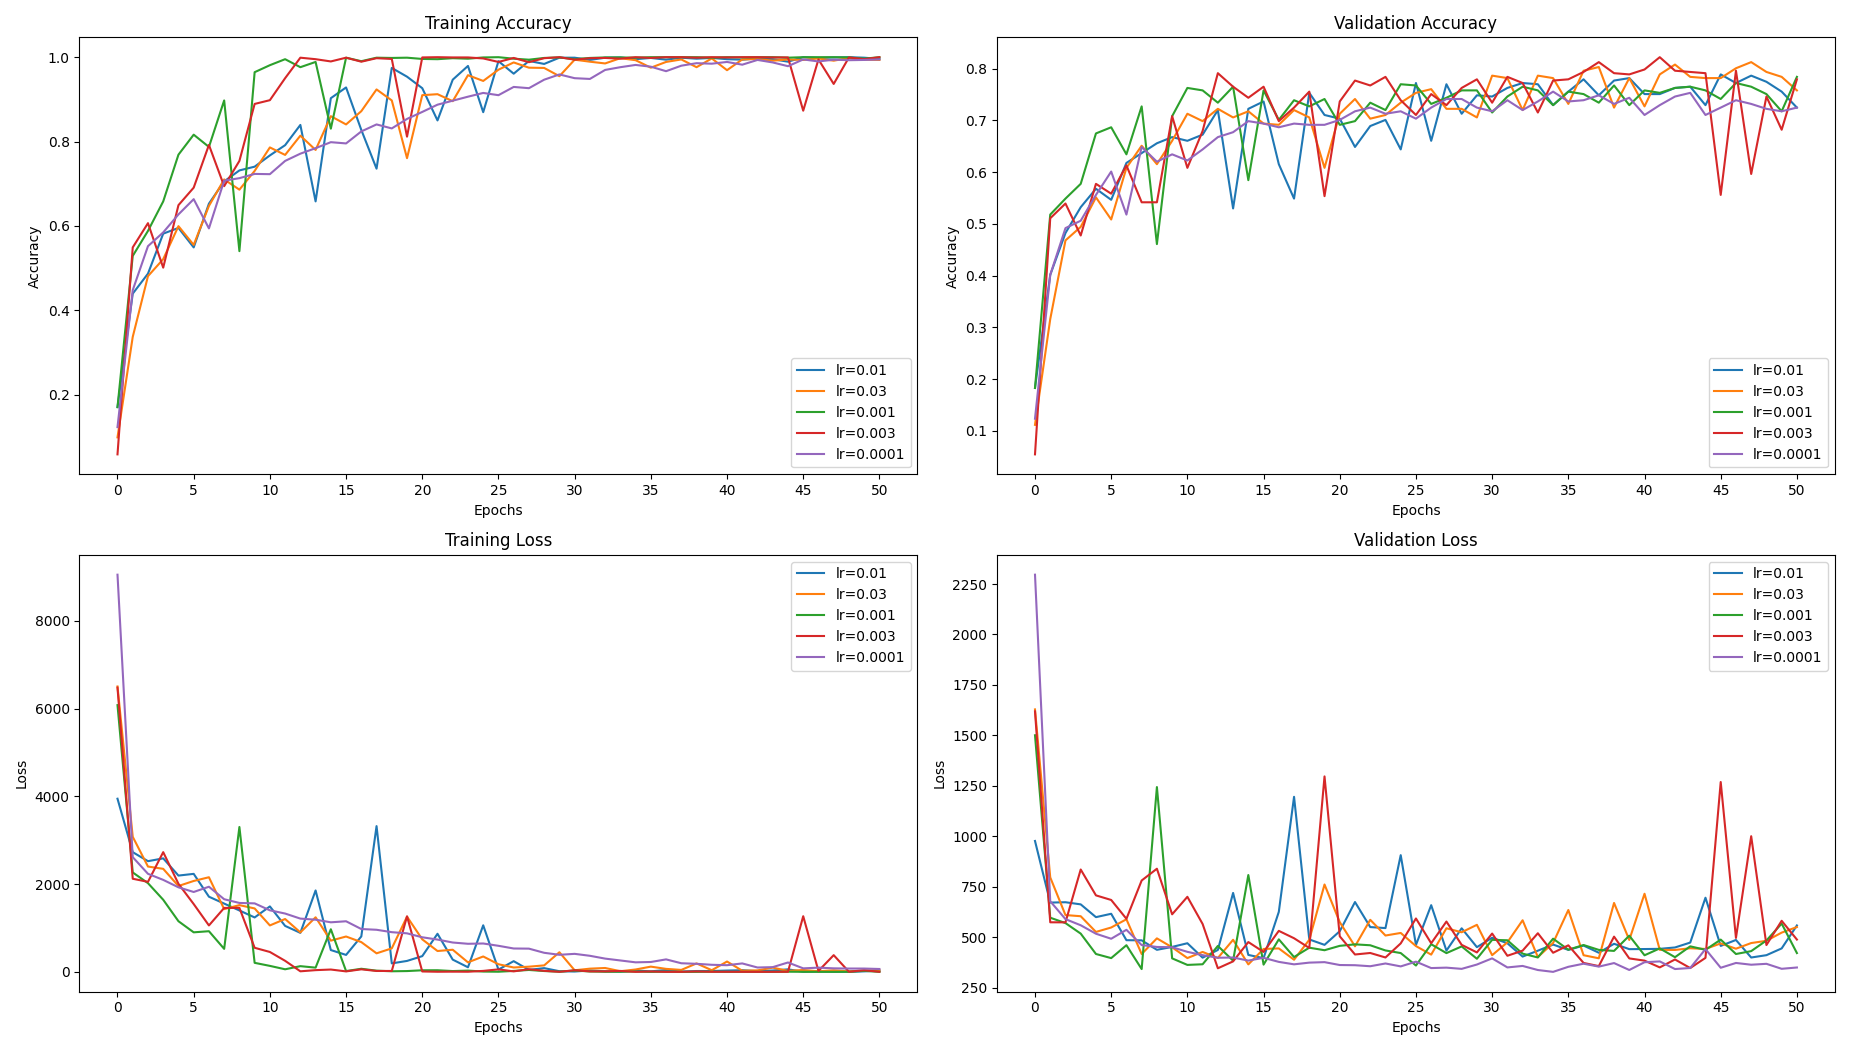
\includegraphics[width=0.9\textwidth]{../out/single_shot_full_model.png}
    \caption{Training the model from scratch on \textit{PACS\_cartoon} dataset}
    \label{fig:full_scratch}
\end{figure}

From the graphs, it can be seen that there is no optimal learning rate $\lambda$ that would work well during the whole optimization.
In the beginning, the larger values are more promising because the loss and accuracy are improving fast but as we approach low loss and high accuracy, the model starts to get slightly worse or fluctuate around a value.
On the other hand, the lowest value $\lambda = 0.0001$ has a nice smooth curve in accuracy and loss but it decreases too slowly for 50 epochs.
This is one of the main arguments for dynamically changing the learning rate in different phases of learning.

From the cross-validation, the best value of the learning rate was $\lambda = 0.003$, which is in the middle of the set and thus it makes sense as a kind of trade-off among the values.
For this learning rate, the best epoch to stop was the epoch $41$.
The evaluation metrics of this model selected based on the best performance on the validation set were as shown in \ref{table:full_model_acc}.

\begin{table}[ht]
    \centering
    \begin{tabular}{ | r | l | }
        \hline
        Learning rate       & $0.003$   \\
        \hline
        Stopping epoch      & $41$      \\
        \hline
        Validation accuracy & $82.19\%$ \\
        \hline
        Test accuracy       & $64.41\%$ \\
        \hline
    \end{tabular}
    \caption{The evaluation metrics of the full model train from scratch}
    \label{table:full_model_acc}
\end{table}

Lastly, we show a few examples of this model incorrect predictions together with the correct class and top-3 predicted classes with probabilities.
These images are shown in figure \ref{fig:full_model_incorrect}.

\begin{figure}[ht]
    \centering
    \begin{subfigure}[b]{0.45\textwidth}
        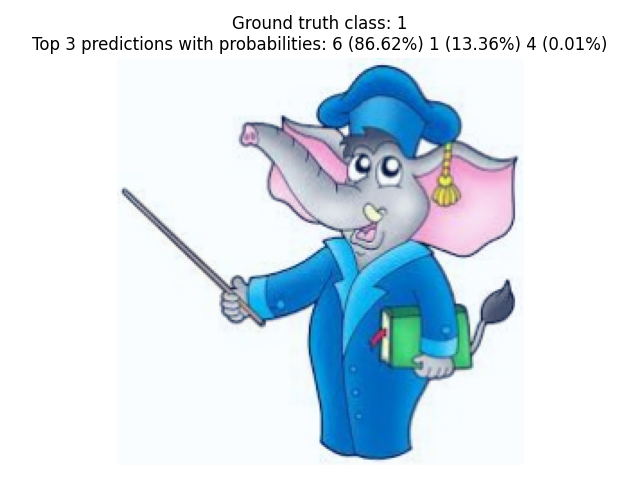
\includegraphics[width=\textwidth]{../out/single_shot_full_model/error_0.png}
    \end{subfigure}
    \hfill
    \begin{subfigure}[b]{0.45\textwidth}
        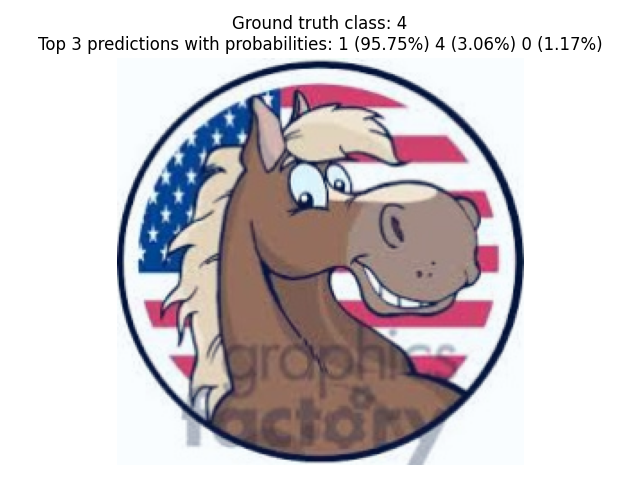
\includegraphics[width=\textwidth]{../out/single_shot_full_model/error_1.png}
    \end{subfigure}
    \begin{subfigure}[b]{0.45\textwidth}
        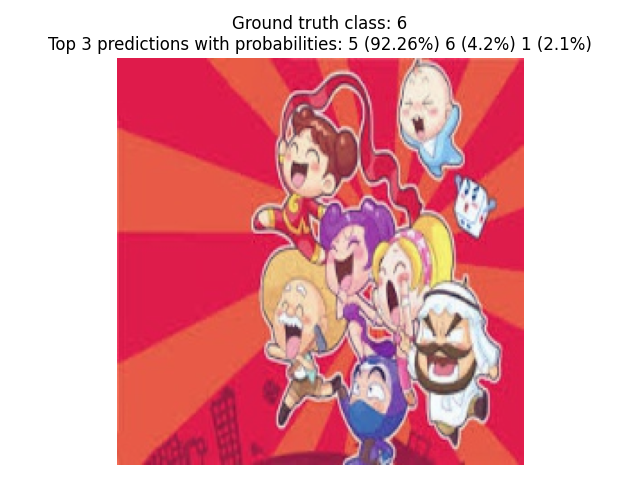
\includegraphics[width=\textwidth]{../out/single_shot_full_model/error_2.png}
    \end{subfigure}
    \hfill
    \begin{subfigure}[b]{0.45\textwidth}
        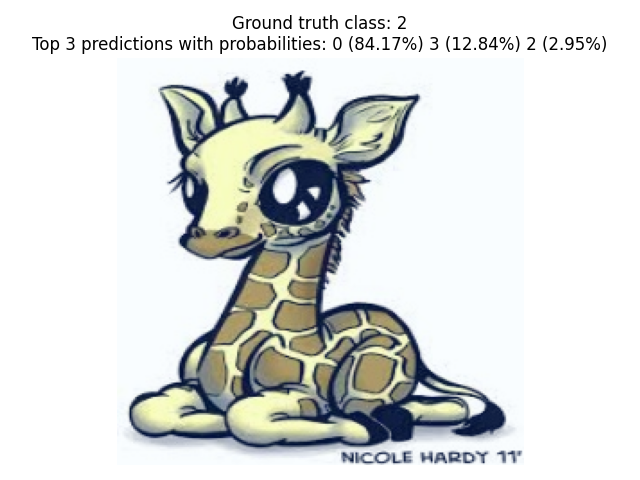
\includegraphics[width=\textwidth]{../out/single_shot_full_model/error_3.png}
    \end{subfigure}
    \caption{Incorrectly classified images by model trained from scratch}
    \label{fig:full_model_incorrect}
\end{figure}

\subsubsection{Fine Tuning}
Previously, we trained the full model from scratch and evaluated the predictor.
To try to improve performance, we will use the same model but with pretrained weights.
Again, we will replace the last classification layer with a new linear layer with $7$ output neurons and intialized again by \textit{xavier} method.
Although we use the pretrained weights, we freeze them so only the weights in the last output layer are trained, not the entire model.

The same hyperparameters were used as in the previous experiment and which are summarized in table \ref{table:hyperparams}.
The dataset was split again in the same way and the seed was set to the same value as in previous task.
Only the model was different.
The summary of results from this type of training is in table \ref{table:fine_tuning_acc}.

\begin{table}[ht]
    \centering
    \begin{tabular}{ | r | l | }
        \hline
        Learning rate       & $0.001$   \\
        \hline
        Stopping epoch      & $13$      \\
        \hline
        Validation accuracy & $89.07\%$ \\
        \hline
        Test accuracy       & $79.67\%$ \\
        \hline
    \end{tabular}
    \caption{The evaluation metrics of the fine-tuned model with frozen weights}
    \label{table:fine_tuning_acc}
\end{table}

\subsubsection{Full Fine Tuning}
This last experiment is the very similar to the previous one but this time the weights are not frozen so we train the whole network with our custom last layer on the cartoon dataset.
The parameters and split are again the same, just as in table \ref{table:hyperparams}.
The results of learning are summarized in table \ref{table:full_fine_tuning_acc}.

\begin{table}[ht]
    \centering
    \begin{tabular}{ | r | l | }
        \hline
        Learning rate       & $0.001$   \\
        \hline
        Stopping epoch      & $35$      \\
        \hline
        Validation accuracy & $97.15\%$ \\
        \hline
        Test accuracy       & $92.80\%$ \\
        \hline
    \end{tabular}
    \caption{The evaluation metrics of the full fine-tuned model}
    \label{table:full_fine_tuning_acc}
\end{table}

\subsubsection{Comparison}
As expected, the last option, fine-tuning pre-trained model without freezing the weights, achieved the highest accuracy of all three options.
Training from scratch would need much more data and time to achieve similar results, but we still were able to learn something even in 50 epochs.
In all cases, some way of adapting the learning rate $\lambda$ during training would probably help to improve the model.
We can observe benefits of all used learning rates from the biggest begin good at reducing the loss quickly at the beginning to the smallest one having the smoothest and most consistent decrease.
This is especially true for the fine tuned models, where the weights are already really good and big learning rate can set the learning back a little as I want to demonstrate on a plot from the full fine-tuning learning in figure \ref{fig:full_fine_tuning}.

\begin{figure}[ht]
    \centering
    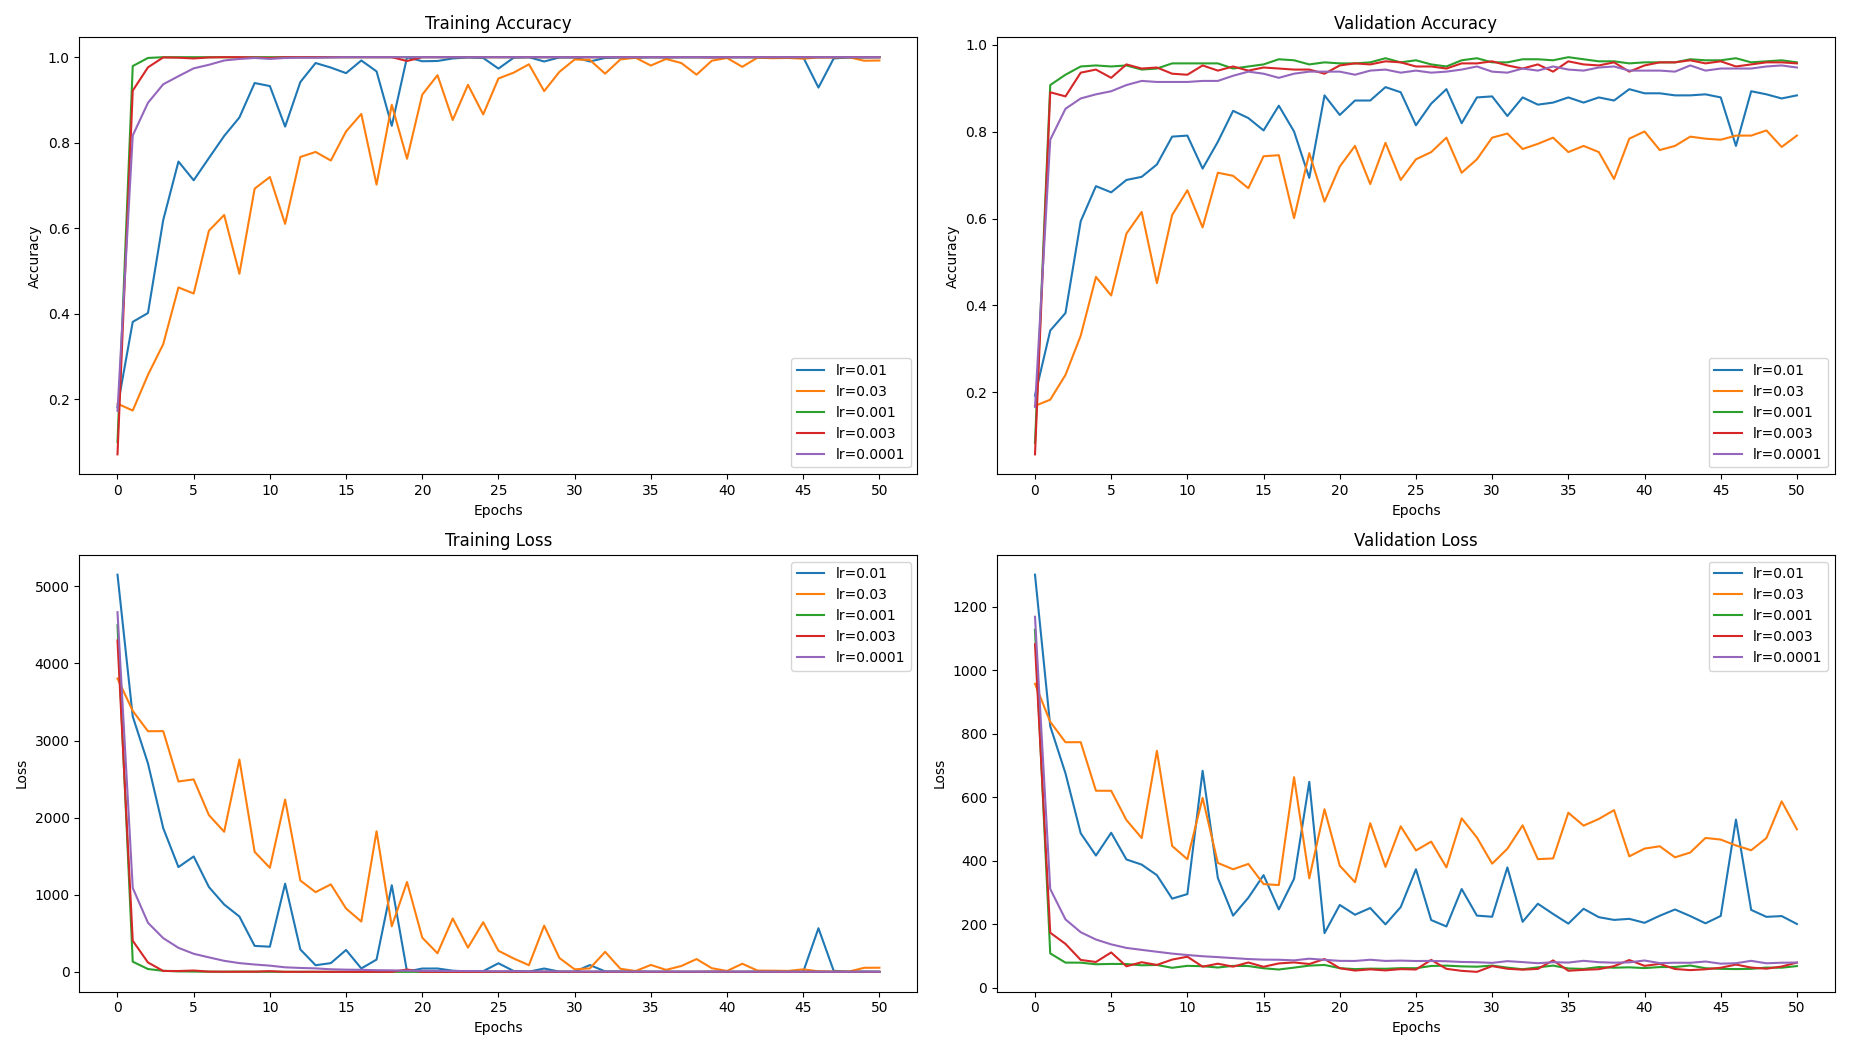
\includegraphics[width=0.9\textwidth]{../out/single_shot_full_fine_tuning.png}
    \caption{Full fine-tuning on \textit{PACS\_cartoon} dataset}
    \label{fig:full_fine_tuning}
\end{figure}

Here, we can clearly see, that in this case the smaller learning rates is much better as it increases the accuracy fast and smoothly in constrast to the bigger learning rates.
However, when we look back at table \ref{fig:full_scratch}, we can see that there the bigger learning rates have its benefits.

\subsection{Few shot PACS cartoon dataset}
Now we are supposed to the the same things as in previous section but on a smaller dataset \textit{PACS\_cartoon\_few\_shot}.

\subsubsection{Preprocessing}
Just out of curiosisty I compare the sizes of the datasets in table \ref{table:dataset_sizes}.

\begin{table}[ht]
    \centering
    \begin{tabular}{| r | c | c |}
        \hline
        Dataset                  & Training set & Test set \\
        \hline
        \hline
        PACS\_cartoon            & $2108$       & $236$    \\
        \hline
        PACS\_cartoon\_few\_shot & $236$        & $2108$   \\
        \hline
    \end{tabular}
    \caption{Sizes of the datasets}
    \label{table:dataset_sizes}
\end{table}

This might be very hard to do since, the training set is so small and we take some portion of it as a validation set, so in training it is even smaller.
Also, it is necessary to recompute the normalization statistics for the new dataset and they are provided in table \ref{table:stats_few_shot}.

\begin{table}[ht]
    \centering
    \begin{tabular}{| r | c | c |}
        \hline
        Dataset                           & Mean                       & Standard Deviation         \\
        \hline
        \hline
        \textbf{PACS\_cartoon\_few\_shot} & $[0.7739, 0.7576, 0.7179]$ & $[0.2972, 0.2968, 0.3353]$ \\
        \hline
        \textbf{PACS\_cartoon}            & $[0.8116, 0.7858, 0.7380]$ & $[0.2730, 0.2863, 0.3374]$ \\
        \hline
        \textbf{ImageNet}                 & $[0.485, 0.456, 0.406]$    & $[0.229, 0.224, 0.225]$    \\
        \hline
    \end{tabular}
    \caption{Statistics of the training set comapred to \textbf{ImageNet}}
    \label{table:stats_few_shot}
\end{table}

\subsubsection{Training from scratch}
The setup of the experiments was exactly the same as with the previous dataset so I will not repeat the training hyperparameters here but refer the reader to table \ref{table:hyperparams}.
The results are shown in a plot \ref{fig:few_shot_scratch} and the final results in \ref{table:few_shot_full_model_acc}.

\begin{table}[ht]
    \centering
    \begin{tabular}{ | r | l | }
        \hline
        Learning rate       & $0.003$   \\
        \hline
        Stopping epoch      & $16$      \\
        \hline
        Validation accuracy & $57.45\%$ \\
        \hline
        Test accuracy       & $49.38\%$ \\
        \hline
    \end{tabular}
    \caption{The evaluation metrics of the model trained from scratch on \textit{PACS\_cartoon\_few\_shot} dataset}
    \label{table:few_shot_full_model_acc}
\end{table}

From the plot we can see that even though the training loss and accuracy are improving, the validation loss is chaotic and does not converge after a point.
This can be a sign of overfitting, where the model can learn perfectly to classify the small training set but does not generalize to the whole dataset.
This is also confirmed by the test accuracy, which is very low.
It can also be the case where the small training set is not very representative of the whole dataset and since the network is not pretrained, it produces terrible results.

\begin{figure}[ht]
    \centering
    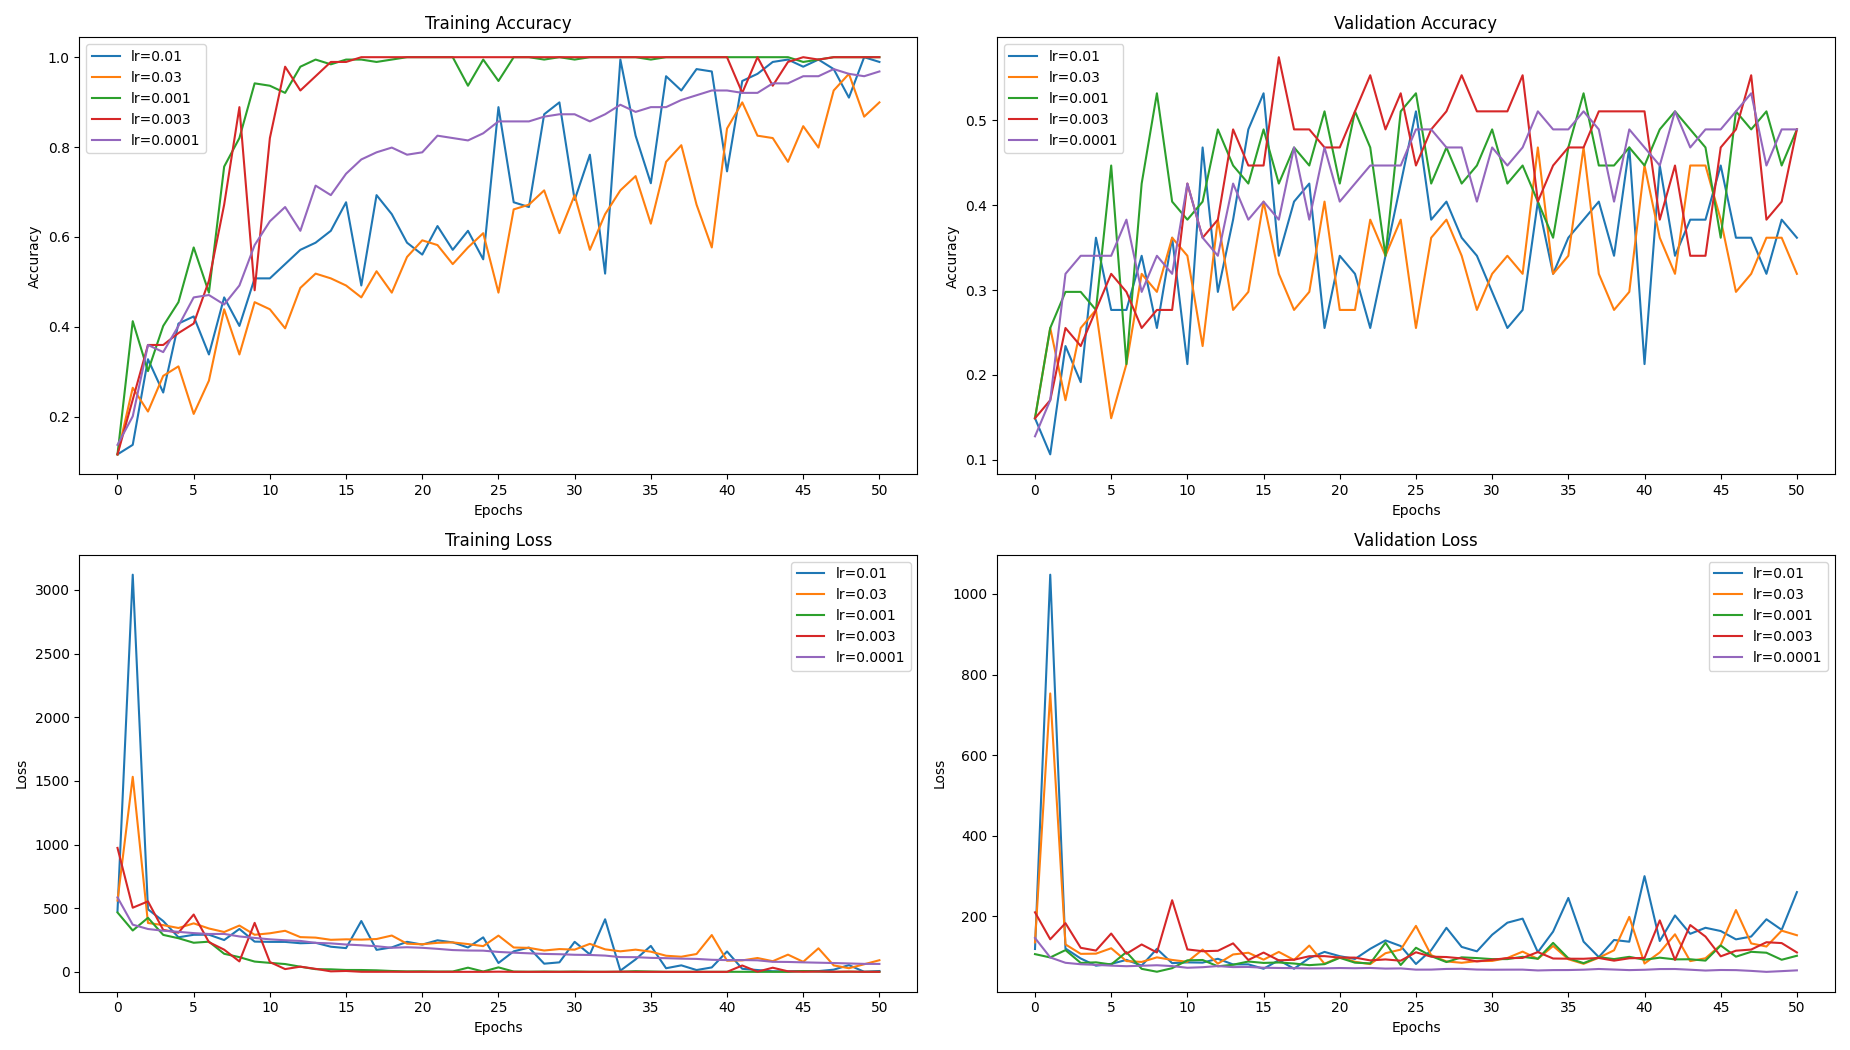
\includegraphics[width=0.9\textwidth]{../out/few_shot_full_model.png}
    \caption{Training the model from scratch on \textit{PACS\_cartoon\_few\_shot} dataset}
    \label{fig:few_shot_scratch}
\end{figure}

Similarly to the first dataset, we show some examples of misclassified images by this network from the test set in figure \ref{fig:few_shot_full_model_incorrect}.
Now, the misclassifications are far less deceiving than in the previous case which corresponds to the phenomena described above.

\begin{figure}[ht]
    \centering
    \begin{subfigure}[b]{0.45\textwidth}
        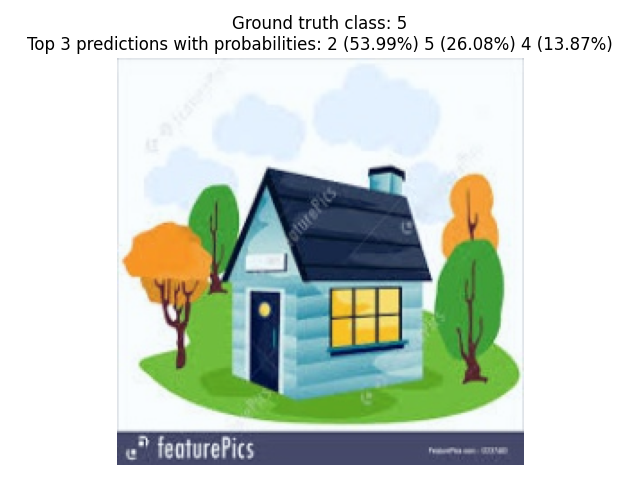
\includegraphics[width=\textwidth]{../out/few_shot_full_model/error_1.png}
    \end{subfigure}
    \hfill
    \begin{subfigure}[b]{0.45\textwidth}
        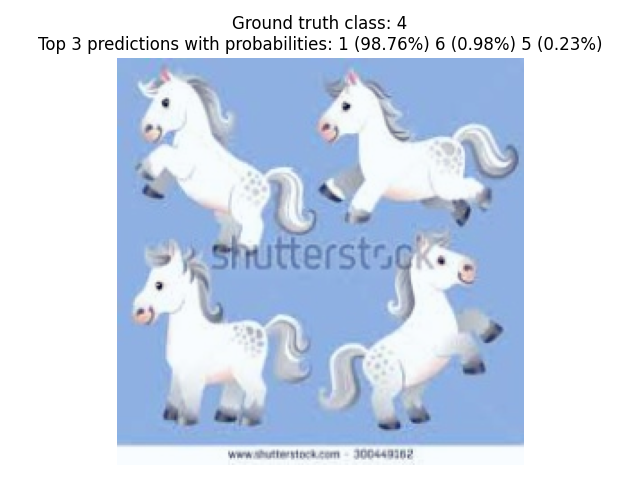
\includegraphics[width=\textwidth]{../out/few_shot_full_model/error_2.png}
    \end{subfigure}
    \begin{subfigure}[b]{0.45\textwidth}
        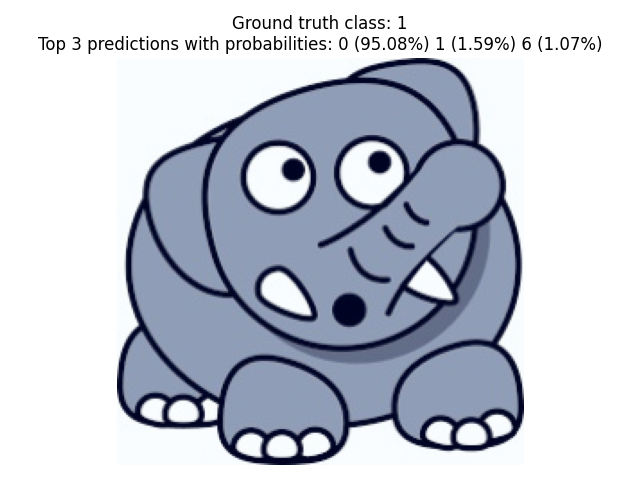
\includegraphics[width=\textwidth]{../out/few_shot_full_model/error_3.png}
    \end{subfigure}
    \hfill
    \begin{subfigure}[b]{0.45\textwidth}
        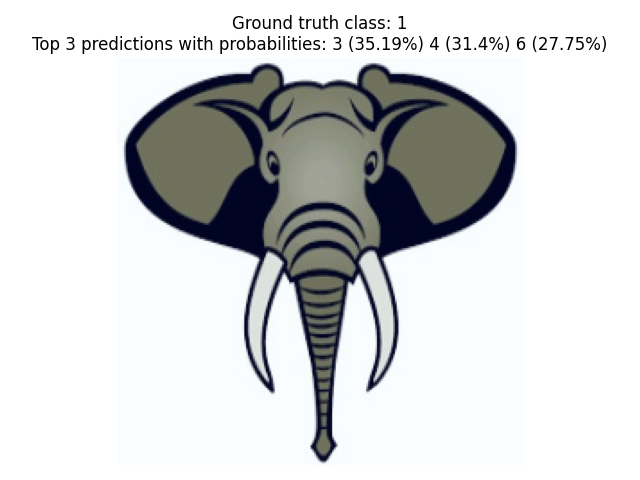
\includegraphics[width=\textwidth]{../out/few_shot_full_model/error_4.png}
    \end{subfigure}
    \caption{Incorrectly classified images by model trained from scratch on \textit{PACS\_cartoon\_few\_shot} dataset}
    \label{fig:few_shot_full_model_incorrect}
\end{figure}

\subsubsection{Fine Tuning}
As with the previous dataset, we freeze the pretrained model and just train the last randomly intialized linear layer.
The results are better than when training from scratch but still not as good as with the bigger dataset.

\begin{table}[ht]
    \centering
    \begin{tabular}{ | r | l | }
        \hline
        Learning rate       & $0.003$   \\
        \hline
        Stopping epoch      & $8$       \\
        \hline
        Validation accuracy & $80.85\%$ \\
        \hline
        Test accuracy       & $68.80\%$ \\
        \hline
    \end{tabular}
    \caption{The evaluation metrics of the fine-tuned model on \textit{PACS\_cartoon\_few\_shot} dataset}
    \label{table:few_shot_fine_tuning_acc}
\end{table}

\subsubsection{Full Fine Tuning}
Now, we again use the pretrained model without freezing the weights and try to fine-tune it as a whole with the new classification linear layer.
The results improved but still could be much higher.
The pretrained weights, probably on a large dataset, can mitigate the lacking size of our learning set, which can be good news when we cannot get many samples but a network is already trained on similar domain.

\begin{table}[ht]
    \centering
    \begin{tabular}{ | r | l | }
        \hline
        Learning rate       & $0.003$   \\
        \hline
        Stopping epoch      & $12$      \\
        \hline
        Validation accuracy & $85.11\%$ \\
        \hline
        Test accuracy       & $81.21\%$ \\
        \hline
    \end{tabular}
    \caption{The evaluation metrics of the fully fine-tuned model on \textit{PACS\_cartoon\_few\_shot} dataset}
    \label{table:few_shot_full_fine_tuning_acc}
\end{table}

\subsubsection{Comparison}
In comparison to the bigger dataset, the results are worse.
However, we can see that the pretrained weights can mitigate it and make the final test error not so low, even though the bigger dataset achieves much higher accuracy.
Training a slightly more deep and complicated network on such a small dataset showed terrible results.
They might be better when the learning rate is dynamically adjusted during learning but still the model is probably just useless.
Much better option is to use transfer learning or, preferably, fine-tuning as demonstrated by the accuracies of the trained predictors.
The training on small dataset is also much less stable than on the other dataset with more fluctuations in accuracy.
In all three options, we see that the training accuracy goes to 1 quickly, but for the small dataset the validation accuracy does not really follow as quickly or at all, while for the bigger dataset it more or less follows the trend of training accuracy and loss.
This could be a sign of overfitting the few training images.

\subsection{Data augmentation}
In this section, we try to apply data augmentation on the small dataset to try and get higher accuracy than in the previous section.
We use the full fine tuning approach.

I sometimes faced with a problem that the validation accuracy was very high, for example $89\%$ but the test accuracy was acutally lower than when the validation accuracy was around $60\%$.
So I experimented with bigger validation set size.

Finally, I managed to improve the classifier slightly by using this set of augmentations:
\begin{verbatim}
transforms.RandomHorizontalFlip(p=0.1),
transforms.RandomAffine(10),
transforms.RandomCrop(200),
transforms.RandomAdjustSharpness(2, p=0.1),
transforms.RandomGrayscale(p=0.1),
\end{verbatim}

Moreover, I increased the validation set size to $0.3$ of the training set and applied the transformations directly on tensors.
I managed to get slightly higher test classification accuracy as shown in table \ref{table:few_shot_augmented_acc}.

\begin{table}[ht]
    \centering
    \begin{tabular}{ | r | l | }
        \hline
        Learning rate       & $0.003$   \\
        \hline
        Stopping epoch      & $41$      \\
        \hline
        Validation accuracy & $87.14\%$ \\
        \hline
        Test accuracy       & $82.54\%$ \\
        \hline
    \end{tabular}
    \caption{The evaluation metrics of the fully fine-tuned model on augmented \textit{PACS\_cartoon\_few\_shot} dataset}
    \label{table:few_shot_augmented_acc}
\end{table}

In conclusion, I did not manage to improve the accuracy significantly, the results are only slightly better.
I think it would required more tuning of the probabilities and transformations to use.
I usually managed to get the training accuracy very close to $1.0$ but the validation accuracy did not always correspond to it.
And when it did, the test accuracy was completely different.
This is not completely unexpected to me since the training set has a size of only $236$ images, from which we must take some to the validation set, and the test set has $2108$ images.
Then we try to estimate the accuracy on $2108$ images from a validation set of size $236 * 0.3 \approx 70$ images so it is not surprising that the test accuracy is lower.

\end{document}
